\documentclass[14pt, a4paper]{extarticle}

\usepackage[margin=1in]{geometry}
\usepackage{graphicx}
\usepackage{enumitem}
\usepackage{multicol}
\usepackage{fancyhdr}
\usepackage{amsfonts}
\usepackage{amssymb}
\usepackage{listings}
\usepackage{float}
\usepackage{wrapfig}

\usepackage{gvv-book}
\usepackage{gvv}

\graphicspath{ {figs/} }

\pagestyle{fancy}
\fancyhf{} 
\fancyhead[L]{2025}
\fancyhead[R]{PH}
\fancyfoot[L]{PH}
\fancyfoot[R]{\thepage/23}
\renewcommand{\headrulewidth}{0.4pt}
\renewcommand{\footrulewidth}{0.4pt}

\let\oldvec\vec
\renewcommand{\vec}[1]{\overrightarrow{#1}}
\newcommand{\myvec}[1]{\begin{bmatrix} #1 \end{bmatrix}}

\begin{document}

\section*{General Aptitude}
\textbf{Q.1 – Q.5 Carry ONE mark Each}

\begin{enumerate}[label=\textbf{Q.\arabic*}]

\item Is there any good show \underline{\hspace{3cm}} television tonight? \\
Select the most appropriate option to complete the above sentence.
\begin{enumerate}
\begin{multicols}{4}
\item in
\item at
\item within
\item on
\end{multicols}
\end{enumerate}
\hfill \textbf{(GATE PH 2025)}

\item As the police officer was found guilty of embezzlement, he was \underline{\hspace{3cm}} dismissed from the service in accordance with the Service Rules. \\
Select the most appropriate option to complete the above sentence.
\begin{enumerate}
\begin{multicols}{2}
\item sumptuously
\item brazenly
\item unintentionally
\item summarily
\end{multicols}
\end{enumerate}
\hfill \textbf{(GATE PH 2025)}

\item The sum of the following infinite series is:
$$ \frac{1}{1!} + \frac{1}{2!} + \frac{1}{3!} + \frac{1}{4!} + \frac{1}{5!} + \dots $$
\begin{enumerate}
\begin{multicols}{4}
\item $\pi$
\item $1+e$
\item $e-1$
\item $e$
\end{multicols}
\end{enumerate}
\hfill \textbf{(GATE PH 2025)}

\item A thin wire is used to construct all the edges of a cube of 1 m side by bending, cutting and soldering the wire. If the wire is 12 m long, what is the minimum number of cuts required to construct the wire frame to form the cube?
\begin{enumerate}
\begin{multicols}{4}
\item 3
\item 4
\item 6
\item 12
\end{multicols}
\end{enumerate}
\hfill \textbf{(GATE PH 2025)}

\item The figures I, II and III are parts of a sequence. Which one of the following options comes next in the sequence at IV?
\begin{figure}[H]
\centering
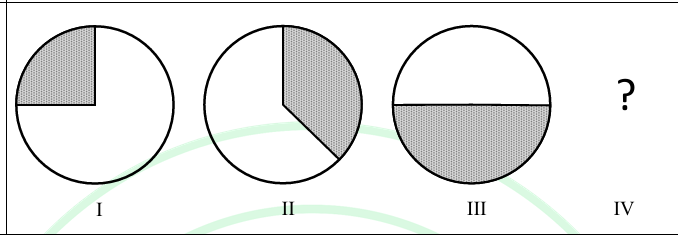
\includegraphics[width=0.7\textwidth]{figs/q3fig25.png}
\caption{A sequence of figures.}
\label{fig:q5_sequence}
\end{figure}
\begin{enumerate}
\item 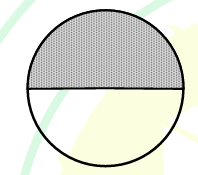
\includegraphics[width=0.25\textwidth]{figs/q3figa25.png}
\item 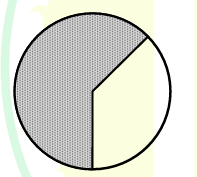
\includegraphics[width=0.25\textwidth]{figs/q3figb25.png}
\item 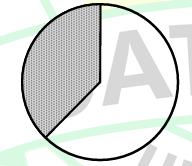
\includegraphics[width=0.25\textwidth]{figs/q3figc25.png}
\item 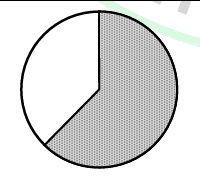
\includegraphics[width=0.25\textwidth]{figs/q3figd25.png}
\end{enumerate}
\hfill \textbf{(GATE PH 2025)}

\end{enumerate}

\textbf{Q.6 – Q.10 Carry TWO marks Each}

\begin{enumerate}[label=\textbf{Q.\arabic*}]

\item
\begin{quote}
“Why do they pull down and do away with crooked streets, I wonder, which are my delight, and hurt no man living? Every day the wealthier nations are pulling down one or another in their capitals and their great towns: they do not know why they do it; neither do I. It ought to be enough, surely, to drive the great broad ways which commerce needs and which are the life-channels of a modern city, without destroying all history and all the humanity in between: the islands of the past.”
\par\raggedleft\textit{(From Hilaire Belloc's “The Crooked Streets”)}
\end{quote}
Based only on the information provided in the above passage, which one of the following statements is true?
\begin{enumerate}
\item The author of the passage takes delight in wondering.
\item The wealthier nations are pulling down the crooked streets in their capitals.
\item In the past, crooked streets were only built on islands.
\item Great broad ways are needed to protect commerce and history.
\end{enumerate}
\hfill \textbf{(GATE PH 2025)}

\item Rohit goes to a restaurant for lunch at about 1 PM. When he enters the restaurant, he notices that the hour and minute hands on the wall clock are exactly coinciding. After about an hour, when he leaves the restaurant, he notices that the clock hands are again exactly coinciding. How much time (in minutes) did Rohit spend at the restaurant?
\begin{enumerate}
\item $64\frac{6}{11}$
\item $66\frac{5}{13}$
\item $65\frac{5}{11}$
\item $66\frac{6}{13}$
\end{enumerate}
\hfill \textbf{(GATE PH 2025)}

\item A color model is shown in the figure with color codes: Yellow (Y), Magenta (M), Cyan (Cy), Red (R), Blue (Bl), Green (G), and Black (K).
\begin{figure}[H]
\centering
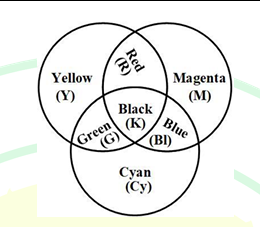
\includegraphics[width=0.3\textwidth]{figs/q8fig25.png}
\caption{A subtractive color model.}
\label{fig:q8_color_model}
\end{figure}
Which one of the following options displays the color codes that are consistent with the color model?
\begin{enumerate}[(A)]
\item 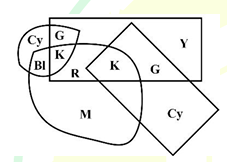
\includegraphics[width=0.5\textwidth]{figs/q8figa25.png}
\item 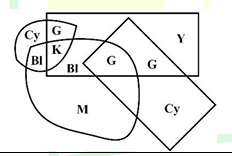
\includegraphics[width=0.5\textwidth]{figs/q8figb25.png}
\item 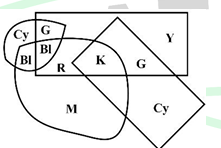
\includegraphics[width=0.5\textwidth]{figs/q8figc25.png}
\item 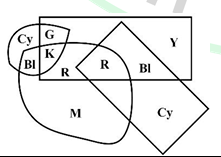
\includegraphics[width=0.5\textwidth]{figs/q8figd25.png}
\end{enumerate}
\hfill \textbf{(GATE PH 2025)}

\item A circle with center at $(x,y) = (0.5, 0)$ and radius = 0.5 intersects with another circle with center at $(x,y) = (1, 1)$ and radius = 1 at two points. One of the points of intersection $(x,y)$ is:
\begin{enumerate}
\begin{multicols}{4}
\item $(0,0)$
\item $(0.2, 0.4)$
\item $(0.5, 0.5)$
\item $(1,2)$
\end{multicols}
\end{enumerate}
\hfill \textbf{(GATE PH 2025)}

\item An object is said to have an $n$-fold rotational symmetry if the object, rotated by an angle of $\frac{2\pi}{n}$ is identical to the original. \\
Which one of the following objects exhibits 4-fold rotational symmetry about an axis perpendicular to the plane of the screen? \\
Note: The figures shown are representative.
\begin{enumerate}
\item 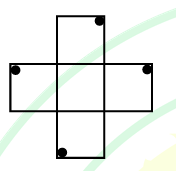
\includegraphics[width=0.3\textwidth]{figs/q10figa25.png}
\item 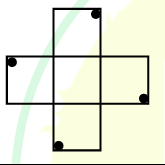
\includegraphics[width=0.3\textwidth]{figs/q10figb25.png}
\item 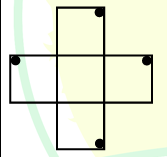
\includegraphics[width=0.3\textwidth]{figs/q10figc25.png}
\item 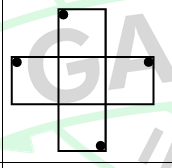
\includegraphics[width=0.3\textwidth]{figs/q10figd25.png}
\end{enumerate}
\hfill \textbf{(GATE PH 2025)}

\end{enumerate}

\textbf{Q.11 – Q.35 Carry ONE mark Each}

\begin{enumerate}[label=\textbf{Q.\arabic*}]

\item For a two-dimensional hexagonal lattice with lattice constant $a$, the atomic density is
\begin{enumerate}
\begin{multicols}{4}
\item $\frac{1}{\sqrt{3}a^2}$
\item $\frac{1}{\sqrt{6}a^2}$
\item $\frac{4}{3\sqrt{3}a^2}$
\item $\frac{1}{3\sqrt{3}a^2}$
\end{multicols}
\end{enumerate}
\hfill \textbf{(GATE PH 2025)}

\item Consider a crystal that has a basis of one atom. Its primitive vectors are $\vec{a_1} = a\hat{i}$, $\vec{a_2} = a\hat{j}$, $\vec{a_3} = \frac{a}{2}(\hat{i} + \hat{j} + \hat{k})$, where $\hat{i}$, $\hat{j}$, $\hat{k}$ are the unit vectors in the $x, y$ and $z$ directions of the Cartesian coordinate system and $a$ is a positive constant. Which one of the following is the correct option regarding the type of the Bravais lattice?
\begin{enumerate}
\item It is BCC and the volume of the primitive cell is $\frac{a^3}{2}$
\item It is FCC and the volume of the primitive cell is $\frac{a^3}{4}$
\item It is BCC and the volume of the primitive cell is $\frac{a^3}{8}$
\item It is FCC and the volume of the primitive cell is $a^3$
\end{enumerate}
\hfill \textbf{(GATE PH 2025)}

\item A particle of mass $m$ is in a potential $V(x) = \frac{1}{2}m\omega^2x^2$ for $x > 0$ and $V(x) = \infty$ for $x \le 0$, where $\omega$ is the angular frequency. The ratio of the energies corresponding to the lowest energy level to the next higher level is
\begin{enumerate}
\begin{multicols}{4}
\item $\frac{3}{7}$
\item $\frac{1}{2}$
\item $\frac{1}{3}$
\item $\frac{3}{5}$
\end{multicols}
\end{enumerate}
\hfill \textbf{(GATE PH 2025)}

\item A particle is scattered from a potential $V(\vec{r}) = g\delta^3(\vec{r})$, where $g$ is a positive constant. Using the first Born approximation, the angular $(\theta, \phi)$ dependence of differential scattering cross section $\frac{d\sigma}{d\Omega}$ is
\begin{enumerate}
\item Independent of $\theta$ but dependent on $\phi$
\item Dependent on $\theta$ but independent of $\phi$
\item Dependent on both $\theta$ and $\phi$
\item Independent of both $\theta$ and $\phi$
\end{enumerate}
\hfill \textbf{(GATE PH 2025)}

\item The Joule-Thomson expansion of a gas is
\begin{enumerate}
\begin{multicols}{4}
\item Isentropic
\item Isenthalpic
\item Isobaric
\item Isochoric
\end{multicols}
\end{enumerate}
\hfill \textbf{(GATE PH 2025)}

\item Which one of the following is correct for the phase velocity $v_p$ and group velocity $v_g$? ($c$ is the speed of light in vacuum)
\begin{enumerate}
\item For matter waves in the relativistic case, $v_p v_g > c^2$
\item For electromagnetic waves in a medium, $v_p$ represents the speed with which energy propagates
\item For electromagnetic waves in a medium, both $v_p$ and $v_g$ can be more than $c$
\item For matter waves in free space, $v_p \neq v_g$
\end{enumerate}
\hfill \textbf{(GATE PH 2025)}

\item As per the Drude model of metals, the electrical resistance of a metallic wire of length $L$ and cross-section area $A$ is \\
(Consider $\tau$ as the relaxation time, $m$ as electron mass, $n$ as carrier concentration and $e$ as electronic charge)
\begin{enumerate}
\begin{multicols}{4}
\item $\frac{mL}{ne^2A\tau}$
\item $\frac{2mL}{ne^2A\tau}$
\item $\frac{mL}{2ne^2A\tau}$
\item $\frac{mL}{4ne^2A\tau}$
\end{multicols}
\end{enumerate}
\hfill \textbf{(GATE PH 2025)}

\item Which one of the following baryons has strangeness quantum number $S = -1$?
\begin{enumerate}
\begin{multicols}{4}
\item $\Sigma^{*0}$
\item $n$
\item $\Xi^{*0}$
\item $\Delta^0$
\end{multicols}
\end{enumerate}
\hfill \textbf{(GATE PH 2025)}

\item As per the Drude model of metals, the electrical resistance of a metallic wire of length $L$ and cross-section area $A$ is \\
(Consider $\tau$ as the relaxation time, $m$ as electron mass, $n$ as carrier concentration and $e$ as electronic charge)
\begin{enumerate}
\begin{multicols}{4}
\item $\frac{mL}{ne^2A\tau}$
\item $\frac{2mL}{ne^2A\tau}$
\item $\frac{mL}{2ne^2A\tau}$
\item $\frac{mL}{4ne^2A\tau}$
\end{multicols}
\end{enumerate}
\hfill \textbf{(GATE PH 2025)}

\item Which one of the following baryons has strangeness quantum number $S = -1$?
\begin{enumerate}
\begin{multicols}{4}
\item $\Sigma^{*0}$
\item $n$
\item $\Xi^{*0}$
\item $\Delta^0$
\end{multicols}
\end{enumerate}
\hfill \textbf{(GATE PH 2025)}

\item A logic gate circuit is shown in the figure below. The correct combination for the input $(P, Q)$ for which the output $T = 1$ is
\begin{figure}[H]
\centering
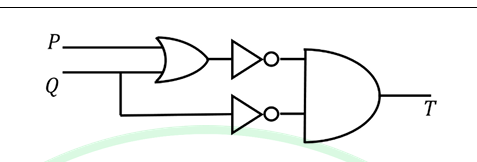
\includegraphics[width=0.4\textwidth]{figs/q19fig25.png}
\caption{Logic gate circuit.}
\label{fig:q19_logic_gate}
\end{figure}
\begin{enumerate}
\begin{multicols}{4}
\item $(0,0)$
\item $(0,1)$
\item $(1,1)$
\item $(1,0)$
\end{multicols}
\end{enumerate}
\hfill \textbf{(GATE PH 2025)}

\item The nuclear energy levels of mirror nuclei are similar. Using this empirical fact alone, the nuclear force can be said to be independent of which one of the following properties of the nucleons?
\begin{enumerate}
\begin{multicols}{4}
\item Mass
\item Spin
\item Charge
\item Parity
\end{multicols}
\end{enumerate}
\hfill \textbf{(GATE PH 2025)}

\item Consider the function $f(z) = \frac{1}{z^2(z-2)^3}$ of a complex variable $z$. The residues of the function at $z=0$ and $z=2$, respectively, are
\begin{enumerate}
\begin{multicols}{4}
\item $-\frac{3}{8}$ and $\frac{3}{8}$
\item $\frac{3}{8}$ and $-\frac{3}{16}$
\item $-\frac{3}{16}$ and $\frac{3}{16}$
\item $-\frac{3}{8}$ and $\frac{3}{16}$
\end{multicols}
\end{enumerate}
\hfill \textbf{(GATE PH 2025)}

\item Consider one mole of a monovalent metal at absolute zero temperature, obeying the free electron model. Its Fermi energy is $E_F$. The energy corresponding to the filling of $\frac{N_A}{2}$ electrons, where $N_A$ is the Avogadro number, is $2^nE_F$. The value of $n$ is
\begin{enumerate}
\begin{multicols}{4}
\item $-\frac{2}{3}$
\item $\frac{2}{3}$
\item $\frac{1}{3}$
\item $-1$
\end{multicols}
\end{enumerate}
\hfill \textbf{(GATE PH 2025)}

\item A paramagnetic material containing paramagnetic ions with total angular momentum $J = \frac{1}{2}$ is kept at absolute temperature $T$. The ratio of the magnetic field required for 80% of the ions to be in the lowest energy state to that required for having 60% of the ions to be in the lowest energy state at the same temperature is
\begin{enumerate}
\item $\frac{2\ln{2}}{\ln\left(\frac{3}{2}\right)}$
\item $\frac{\ln{2}}{\ln\left(\frac{3}{2}\right)}$
\item $\frac{3\ln{2}}{\ln\left(\frac{3}{2}\right)}$
\item $\frac{\ln{3}}{\ln\left(\frac{3}{2}\right)}$
\end{enumerate}
\hfill \textbf{(GATE PH 2025)}

\item Which of the following option(s) is/are correct for the ground state of a hydrogen atom?
\begin{enumerate}
\item Linear Stark effect is zero
\item It has definite parity
\item Spin-orbit coupling is zero
\item Hyperfine splitting is zero
\end{enumerate}
\hfill \textbf{(GATE PH 2025)}

\item Which of the following option(s) is/are correct for photons?
\begin{enumerate}
\item Its rest mass is zero, but its energy is non-zero
\item It carries non-zero linear momentum
\item It carries zero spin angular momentum
\item It has two linearly independent states of polarization
\end{enumerate}
\hfill \textbf{(GATE PH 2025)}

\item A schematic Pressure-Temperature diagram of water is shown in the figure. Which of the following option(s) is/are correct?
\begin{figure}[H]
\centering
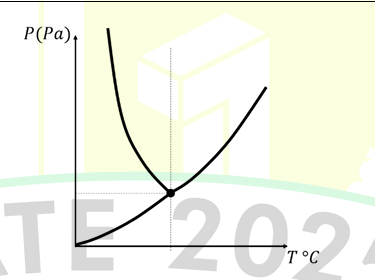
\includegraphics[width=0.3\textwidth]{figs/q26fig25.png}
\caption{P-T diagram for water.}
\label{fig:q26_pt_diagram}
\end{figure}
\begin{enumerate}
\item Clausius-Clapeyron equation is valid across the melting curve and the vaporization curve
\item Melting curve has the highest slope
\item The critical point exists only for the vaporization curve
\item Clausius-Clapeyron equation is not valid across the melting curve and the vaporization curve
\end{enumerate}
\hfill \textbf{(GATE PH 2025)}

\item Which of the following consideration(s) is/are showing that nuclear beta decay, $n \to p + e^- + \bar{\nu}_e$, has to be a three-body decay?
\begin{enumerate}
\item Continuous distribution of the electron energy
\item Spin of the final state
\item Mass of the electron
\item Mass of the proton
\end{enumerate}
\hfill \textbf{(GATE PH 2025)}

\item Potential energy of two diatomic molecules P and Q of the same reduced mass is shown in the figure. According to this diagram, which of the following option(s) is/are correct?
\begin{figure}[H]
\centering
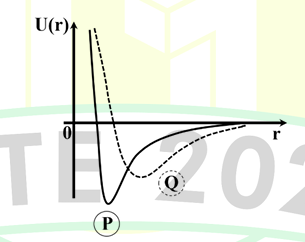
\includegraphics[width=0.3\textwidth]{figs/q28fig25.png}
\caption{Potential energy diagram for two diatomic molecules.}
\label{fig:q28_potential_energy}
\end{figure}
\begin{enumerate}
\item The equilibrium inter-nuclear distance of Q is more than that of P
\item The total energy $E=0$ separates bound and unbound states of the molecules
\item The lowest vibrational frequency of P is larger than that of Q
\item Dissociation energy of Q is more than that of P
\end{enumerate}
\hfill \textbf{(GATE PH 2025)}

\item Nuclear radiation emitted from a $^{60}$Co radioactive source is detected by a photomultiplier tube (PMT) coupled to a scintillator crystal. Which of the following option(s) is/are correct?
\begin{enumerate}
\item $\gamma$ radiation from $^{60}$Co will directly hit the photocathode of the PMT without interacting with the scintillator crystal and produce a signal
\item $\beta$ radiation from $^{60}$Co source interacts with the scintillator crystal, producing $\gamma$ radiation, which will hit the photocathode of the PMT and produce a signal
\item A mu-metal shield is put all around the PMT to nullify the effect of external electric fields
\item A mu-metal shield is put all around the PMT to nullify the effect of external magnetic fields
\end{enumerate}
\hfill \textbf{(GATE PH 2025)}

\item One mole of an ideal monatomic gas at absolute temperature $T$ undergoes free expansion to double its original volume, so that the entropy change is $\Delta S_1$. An identical amount of the same gas at absolute temperature $2T$ undergoes isothermal expansion to double its original volume, so that the entropy change is $\Delta S_2$. The value of $\frac{\Delta S_1}{\Delta S_2}$ (in integer) is \underline{\hspace{3cm}}.
\hfill \textbf{(GATE PH 2025)}

\item A linear dielectric sphere of radius $R$ has a uniform frozen-in polarization along the z-axis. The center of the sphere initially coincides with the origin, about which the electric dipole moment is $\vec{p}_1$. When the sphere is shifted to the point $(2R, 0, 0)$, the corresponding dipole moment with respect to the origin is $\vec{p}_2$. The value of $\frac{|\vec{p}_2|}{|\vec{p}_1|}$ (in integer) is \underline{\hspace{3cm}}.
\hfill \textbf{(GATE PH 2025)}

\item The effective magnetic moment (in units of Bohr magneton) for the ground state of an isolated $4f^6$ ion with 6 unpaired electrons in the $4f$ shell according to Hund's rules is (in integer) \underline{\hspace{3cm}}.
\hfill \textbf{(GATE PH 2025)}

\item Powder X-ray diffraction pattern of a cubic solid with lattice constant $a$ has the (111) diffraction peak at $\theta = 30^{\circ}$. If the lattice expands such that the lattice constant becomes $1.25a$, the angle (in degrees) corresponding to the (111) peak changes to $\sin^{-1}\left(\frac{1}{n}\right)$. The value of $n$ (rounded off to one decimal place) is \underline{\hspace{3cm}}.
\hfill \textbf{(GATE PH 2025)}

\item Consider a monatomic chain of length 30 cm. The phonon density of states is $1.2 \times 10^{-4}$ s. Assuming the Debye model, the velocity of sound in m/s (rounded off to one decimal place) is \underline{\hspace{3cm}}.
\hfill \textbf{(GATE PH 2025)}

\item The $\Delta^+$ baryon with spin $\frac{3}{2}$, at rest, decays to a proton and a pion ($\Delta^+ \to p + \pi^0$). The $\Delta^+$ has positive intrinsic parity and $\pi^0$ has negative intrinsic parity. The orbital angular momentum of the proton-pion system (in integer) is \underline{\hspace{3cm}}.
\end{enumerate}
\hfill \textbf{(GATE PH 2025)}

\textbf{Q.36 – Q.55 Carry TWO marks Each}

\begin{enumerate}[label=\textbf{Q.\arabic*}]

\item The screened nuclear charge of neutral Helium atom is given as $1.7e$, where $e$ is the magnitude of the electronic charge. Assuming the Bohr model of the atom for which the energy levels are $E_n = -\frac{Z^2}{2}\frac{1}{n^2}$ atomic units (Z is the atomic number), the first ionization potential of Helium in atomic units is
\begin{enumerate}
\begin{multicols}{4}
\item 0.89
\item 1.78
\item 0.94
\item 3.16
\end{multicols}
\end{enumerate}
\hfill \textbf{(GATE PH 2025)}

\item The wire loop shown in the figure carries a steady current $I$. Each straight section of the loop has length $d$. A part of the loop lies in $xy$ plane and the other part is tilted at $30^{\circ}$ with respect to the $xz$ plane. The magnitude of the magnetic dipole moment of the loop (in appropriate units) is
\begin{figure}[H]
\centering
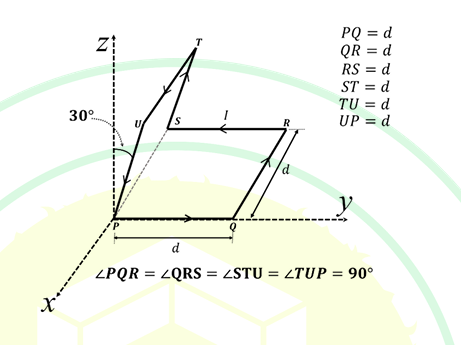
\includegraphics[width=0.5\textwidth]{figs/q37fig25.png}
\caption{A current-carrying wire loop.}
\label{fig:q37_wire_loop}
\end{figure}
\begin{enumerate}
\begin{multicols}{4}
\item $\sqrt{2}Id^2$
\item $2Id^2$
\item $\sqrt{3}Id^2$
\item $Id^2$
\end{multicols}
\end{enumerate}
\hfill \textbf{(GATE PH 2025)}

\item The figure shows a system of two equal masses $m$ and three massless horizontal springs with spring constants $k_1, k_2, k_1$. Ignore gravity. The masses can move only in the horizontal direction and there is no dissipation. If $m=1, k_1=2$ and $k_2=3$ (all in appropriate units), the frequencies of the normal modes of the system in the same system of units are
\begin{figure}[H]
\centering
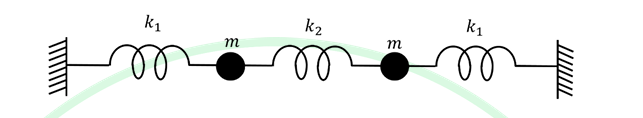
\includegraphics[width=0.6\textwidth]{figs/q38fig25.png}
\caption{A coupled mass-spring system.}
\label{fig:q38_mass_spring}
\end{figure}
\begin{enumerate}
\begin{multicols}{4}
\item $\sqrt{2}, \sqrt{8}$
\item $\sqrt{2}, \sqrt{6}$
\item $\sqrt{3}, \sqrt{10}$
\item $\sqrt{3}, \sqrt{8}$
\end{multicols}
\end{enumerate}
\hfill \textbf{(GATE PH 2025)}

\item Two projectile protons $P_1$ and $P_2$ both with spin up (along the $+z$ direction) are scattered from another fixed target proton $T$ with spin up at rest in the $xy$ plane, as shown in the figure. They scatter one at a time. The nuclear interaction potential between both the projectiles and the target proton is $\lambda\vec{L}\cdot\vec{S}$, where $\vec{L}$ is the orbital angular momentum of the system with respect to the target, $\vec{S}$ is the spin angular momentum of the system and $\lambda$ is a negative constant in appropriate units. Which one of the following is correct?
\begin{figure}[H]
\centering
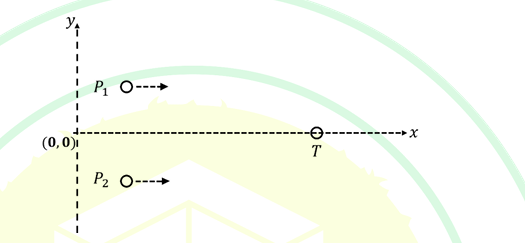
\includegraphics[width=0.5\textwidth]{figs/q39fig25.png}
\caption{Proton-proton scattering.}
\label{fig:q39_proton_scattering}
\end{figure}
\begin{enumerate}
\item $P_1$ will be scattered in the $+y$ direction (upward) and $P_2$ will be scattered in the $-y$ direction (downward)
\item $P_1$ will be scattered in the $+y$ direction (upward) and $P_2$ will be scattered in the $+y$ direction (upward)
\item $P_1$ will be scattered in the $-y$ direction (downward) and $P_2$ will be scattered in the $+y$ direction (upward)
\item $P_1$ will be scattered in the $-y$ direction (downward) and $P_2$ will be scattered in the $-y$ direction (downward)
\end{enumerate}
\hfill \textbf{(GATE PH 2025)}

\item A thin circular ring of radius $R$ lies in the $xy$ plane with its centre coinciding with the origin. The ring carries a uniform line charge density $\lambda$. The quadrupole contribution to the electrostatic potential at the point $(0, 0, d)$, where $d \gg R$, is
\begin{enumerate}
\begin{multicols}{4}
\item $-\frac{\lambda R^3}{4\epsilon_0 d^3}$
\item $0$
\item $\frac{\lambda R^3}{4\epsilon_0 d^3}$
\item $-\frac{\lambda R^3}{2\epsilon_0 d^3}$
\end{multicols}
\end{enumerate}
\hfill \textbf{(GATE PH 2025)}

\item An $\alpha$ particle is scattered from an Au target at rest as shown in the figure. $D_1$ and $D_2$ are the detectors to detect the scattered $\alpha$ particle at an angle $\theta$ and along the beam direction, respectively, as shown. The signals from $D_1$ and $D_2$ are converted to logic signals and fed to logic gates. When a particle is detected, the signal is 1 and is 0 otherwise. Which one of the following circuits detects the particle scattered at the angle $\theta$ only?
\begin{figure}[H]
\centering
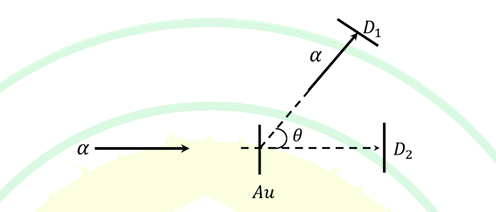
\includegraphics[width=0.6\textwidth]{figs/q41fig25.png}
\caption{Scattering experiment setup.}
\label{fig:q41_scattering}
\end{figure}
\begin{enumerate}[(A)]
\item 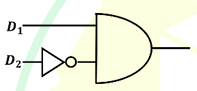
\includegraphics[width=0.4\textwidth]{figs/q41figa25.png}
\item 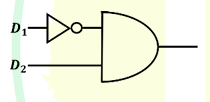
\includegraphics[width=0.4\textwidth]{figs/q41figb25.png}
\item 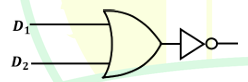
\includegraphics[width=0.4\textwidth]{figs/q41figc25.png}
\item 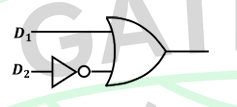
\includegraphics[width=0.4\textwidth]{figs/q41figd21.png}
\end{enumerate}
\hfill \textbf{(GATE PH 2025)}

\item Consider a two-level system with energy states $+\epsilon$ and $-\epsilon$. The number of particles at $+\epsilon$ level is $N_+$ and the number of particles at $-\epsilon$ level is $N_-$. The total energy of the system is $E$ and the total number of particles is $N = N_+ + N_-$. In the thermodynamic limit, the inverse of the absolute temperature of the system is \\
(Given: $\ln N! \approx N\ln N - N$)
\begin{enumerate}
\item $\frac{k_B}{2\epsilon}\ln\left[\frac{N-\frac{E}{\epsilon}}{N+\frac{E}{\epsilon}}\right]$
\item $\frac{k_B}{\epsilon}\ln N$
\item $\frac{k_B}{2\epsilon}\ln N$
\item $\frac{k_B}{\epsilon}\ln\left[\frac{N-\frac{E}{\epsilon}}{N+\frac{E}{\epsilon}}\right]$
\end{enumerate}
\hfill \textbf{(GATE PH 2025)}

\item Let $|m\rangle$ and $|n\rangle$ denote the energy eigenstates of a one-dimensional simple harmonic oscillator. The position and momentum operators are $\hat{X}$ and $\hat{P}$, respectively. The matrix element $\langle m|\hat{P}\hat{X}|n\rangle$ is non-zero when
\begin{enumerate}
\begin{multicols}{4}
\item $m = n \pm 2$ only
\item $m = n$ or $m = n \pm 2$
\item $m = n \pm 3$ only
\item $m = n \pm 1$ only
\end{multicols}
\end{enumerate}
\hfill \textbf{(GATE PH 2025)}

\item A two-level quantum system has energy eigenvalues $E_1$ and $E_2$. A perturbing potential $H' = \lambda\Delta\sigma_x$ is introduced, where $\Delta$ is a constant having dimensions of energy, $\lambda$ is a small dimensionless parameter, and $\sigma_x = \begin{pmatrix} 0 & 1 \\ 1 & 0 \end{pmatrix}$. The magnitudes of the first and the second order corrections to $E_1$ due to $H'$, respectively, are
\begin{enumerate}
\item $0$ and $\frac{\lambda^2\Delta^2}{|E_1-E_2|}$
\item $\frac{|\lambda\Delta|}{2}$ and $\frac{\lambda^2\Delta^2}{|E_1-E_2|}$
\item $|\lambda\Delta|$ and $\frac{\lambda^2\Delta^2}{|E_1-E_2|}$
\item $0$ and $\frac{1}{2}\frac{\lambda^2\Delta^2}{|E_1-E_2|}$
\end{enumerate}
\hfill \textbf{(GATE PH 2025)}

\item An electron with mass $m$ and charge $q$ is in the spin up state $\begin{pmatrix} 1 \\ 0 \end{pmatrix}$ at time $t=0$. A constant magnetic field is applied along the y-axis, $B = B_0\hat{j}$, where $B_0$ is a constant. The Hamiltonian of the system is $H = -\hbar\omega\sigma_y$, where $\omega = \frac{qB_0}{2m} > 0$ and $\sigma_y = \begin{pmatrix} 0 & -i \\ i & 0 \end{pmatrix}$. The minimum time after which the electron will be in the spin down state along the x-axis, i.e., $\frac{1}{\sqrt{2}}\begin{pmatrix} 1 \\ -1 \end{pmatrix}$, is
\begin{enumerate}
\begin{multicols}{4}
\item $\frac{\pi}{8\omega}$
\item $\frac{\pi}{4\omega}$
\item $\frac{\pi}{2\omega}$
\item $\frac{\pi}{\omega}$
\end{multicols}
\end{enumerate}
\hfill \textbf{(GATE PH 2025)}

\item A system of three non-identical spin $\frac{1}{2}$ particles has the Hamiltonian $H = \frac{A}{\hbar^2}(\vec{S}_1 + \vec{S}_2)\cdot\vec{S}_3$, where $\vec{S}_1, \vec{S}_2$ and $\vec{S}_3$ are the spin operators of particles labelled 1, 2 and 3 respectively and $A$ is a constant with appropriate dimensions. The set of possible energy eigenvalues of the system is
\begin{enumerate}
\begin{multicols}{4}
\item $0, \frac{A}{2}, -A$
\item $0, \frac{A}{2}, -\frac{A}{2}$
\item $0, -\frac{3A}{2}, -\frac{A}{2}$
\item $0, -\frac{3A}{2}, \frac{A}{2}$
\end{multicols}
\end{enumerate}
\hfill \textbf{(GATE PH 2025)}

\item Which of the following option(s) is/are correct for a Type I superconductor?
\begin{enumerate}
\item The phase transition to the normal state in the absence of a magnetic field is of second order
\item With increase in temperature, the critical magnetic field decreases linearly to zero
\item Below the critical temperature, the entropy in the superconducting state is less than that in the normal state
\item The phase transition to the normal state in the presence of a magnetic field is of first order
\end{enumerate}
\hfill \textbf{(GATE PH 2025)}

\item Consider two hypothetical nuclei $X_1$ and $X_2$ undergoing $\beta$ decay, resulting in nuclei $Y_1$ and $Y_2$, respectively. The decay scheme and the corresponding $J^P$ values of the nuclei are given in the figure. Which of the following option(s) is/are correct? ($J$ is the total angular momentum and $P$ is parity)
\begin{figure}[H]
\centering
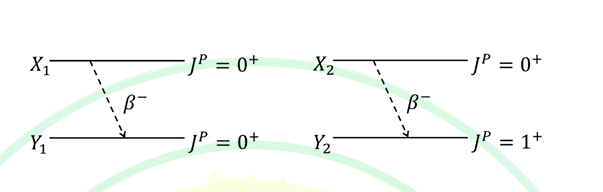
\includegraphics[width=0.7\textwidth]{figs/q48fig25.png}
\caption{Beta decay schemes for nuclei X1 and X2.}
\label{fig:q48_beta_decay}
\end{figure}
\begin{enumerate}
\item $X_1 \to Y_1$ is Fermi transition and $X_2 \to Y_2$ is Fermi transition
\item $X_1 \to Y_1$ is Fermi transition and $X_2 \to Y_2$ is Gamow-Teller transition
\item $X_1 \to Y_1$ is Gamow-Teller transition and $X_2 \to Y_2$ is Fermi transition
\item $X_1 \to Y_1$ is Gamow-Teller transition and $X_2 \to Y_2$ is Gamow-Teller transition
\end{enumerate}
\hfill \textbf{(GATE PH 2025)}

\item A point charge $q$ is placed at a distance $d$ above an infinite, grounded conducting plate placed on the $xy$ plane at $z=0$. The electrostatic potential in $z>0$ region is given by $\phi = \phi_1 + \phi_2$, where $\phi_1 = \frac{1}{4\pi\epsilon_0}\frac{q}{\sqrt{x^2+y^2+(z-d)^2}}$ and $\phi_2 = -\frac{1}{4\pi\epsilon_0}\frac{q}{\sqrt{x^2+y^2+(z+d)^2}}$. Which of the following option(s) is/are correct?
\begin{enumerate}
\item The magnitude of the force experienced by the point charge $q$ is $\frac{1}{16\pi\epsilon_0}\frac{q}{d^2}$
\item The electrostatic energy of the system is $\frac{1}{8\pi\epsilon_0}\frac{q^2}{d}$
\item The induced surface charge density on the plate is proportional to $\frac{1}{\sqrt{x^2+y^2+d^2}}$
\item The electrostatic potential $\phi_1$ satisfies Poisson's equation for $z > 0$
\end{enumerate}
\hfill \textbf{(GATE PH 2025)}

\item In coordinates $(t, x)$, a contravariant second rank tensor $A$ has non-zero diagonal components $A^{tt} = P$ and $A^{xx} = Q$, with all other components vanishing, and $P, Q$ being real constants. Here, $t$ is time and $x$ is space coordinate. Consider a Lorentz transformation $(t, x) \to (t', x')$ to another frame that moves with relative speed $v$ in the $+x$ direction, so that $A \to A'$. If $A'^{tt}$ and $A'^{xx}$ are the diagonal components of $A'$, then setting the speed of light $c=1$, and with $\gamma = \frac{1}{\sqrt{1-v^2}}$, which of the following option(s) is/are correct?
\begin{enumerate}
\item $A'^{tt} = \gamma^2 P + \gamma^2 v^2 Q$
\item $A'^{tt} = \gamma^2 v^2 P + \gamma^2 Q$
\item $A'^{xx} = \gamma^2 v^2 P + \gamma^2 Q$
\item $A'^{xx} = \gamma^2 P + \gamma^2 v^2 Q$
\end{enumerate}
\hfill \textbf{(GATE PH 2025)}

\item The Lagrangian of a particle of mass $m$ and charge $q$ moving in a uniform magnetic field of magnitude $2B$ that points in the $z$ direction, is given by $L = \frac{m}{2}v^2 + qB(xv_y - yv_x)$ where $v_x, v_y, v_z$ are the components of its velocity $\vec{v}$. If $p_x, p_y, p_z$ denote the conjugate momenta in the $x,y,z$ directions and $H$ is the Hamiltonian, which of the following option(s) is/are correct ?
\begin{enumerate}
\item $\frac{dx}{dt} = \frac{1}{m}(p_x - qBy)$
\item $\frac{dp_x}{dt} = \frac{qB}{m}(p_y - qBx)$
\item $\frac{dp_y}{dt} = -\frac{qB}{m}(p_x + qBy)$
\item $H = \frac{1}{2m}[(p_x + qBy)^2 + (p_y - qBx)^2 + p_z^2]$
\end{enumerate}
\hfill \textbf{(GATE PH 2025)}

\item A bead is constrained to move along a long, massless, frictionless horizontal rod parallel to the x axis. The rod itself is moving vertically upward along the z direction against gravity with a constant speed, starting from $z=0$ at $t=0$, and remains horizontal. The conjugate momenta are denoted by $p_x, p_y, p_z$ and the Hamiltonian by $H$. Which of the following option(s) is/are correct?
\begin{enumerate}
\item $H$ is the total energy of the system and is conserved
\item $H$ is the total energy of the system and is not conserved
\item $H$ is not the total energy of the system, but it is conserved
\item $H$ is not the total energy of the system and is not conserved
\end{enumerate}
\hfill \textbf{(GATE PH 2025)}

\item In a one-dimensional Hamiltonian system with position $q$ and momentum $p$, consider the canonical transformation $(q, p) \to (Q = \frac{1}{p}, P = qp^2)$, where $Q$ and $P$ are the new position and momentum, respectively. Which of the following option(s) regarding the generating function $F$ is/are correct?
\begin{enumerate}
\item $F = F_1(q,Q) = \frac{q}{Q}$
\item $F = F_2(q,P) = \sqrt{Pq}$
\item $F = F_3(p,Q) = 2\frac{p}{Q}$
\item $F = F_4(p,P) = \frac{P}{p}$
\end{enumerate}
\hfill \textbf{(GATE PH 2025)}

\item The energy of a free, relativistic particle of rest mass $m$ moving along the $x$ axis in one dimension, is denoted by $T$. When moving in a given potential $V(x)$, its Hamiltonian is $H = T + V(x)$. In the presence of this potential, its speed is $v$, conjugate momentum $p$, and the Lagrangian $L$. Then, which of the following option(s) is/are correct?
\begin{enumerate}
\item $H = c\sqrt{m^2 + \frac{p^2}{c^2}} + V(x)$
\item $v = \frac{pc}{\sqrt{p^2+m^2c^2}}$
\item $L = mc^2\sqrt{1-\frac{v^2}{c^2}} - V(x)$
\item $L = -mc^2\sqrt{1-\frac{v^2}{c^2}} - V(x)$
\end{enumerate}
\hfill \textbf{(GATE PH 2025)}

\item Consider the integral
$$ I = \frac{1}{2\pi i}\oint \frac{z^4-1}{\left(z-\frac{a}{b}\right)\left(z-\frac{b}{a}\right)}dz, $$
where z is a complex variable and $a, b$ are positive real numbers. The integral is taken over a unit circle with center at the origin. Which of the following option(s) is/are correct?
\begin{enumerate}
\item $I = \frac{5}{8}$ when $a=1, b=2$
\item $I = \frac{10}{3}$ when $a=1, b=3$
\item $I = \frac{5}{8}$ when $a=2, b=1$
\item $I = \frac{5}{8}$ when $a=3, b=2$
\end{enumerate}
\hfill \textbf{(GATE PH 2025)}

\item A neutral conducting sphere of radius $R$ is placed in a uniform electric field of magnitude $E_0$, that points along the z axis. The electrostatic potential at any point $\vec{r}$ outside the sphere is given by $V(r, \theta) = V_0 - E_0r\left(1-\frac{R^3}{r^3}\right)\cos\theta$, where $V_0$ is the constant potential of the sphere. Which of the following option(s) is/are correct?
\begin{enumerate}
\item The induced surface charge density on the sphere is proportional to $\sin\theta$
\item As $r \to \infty$, $\vec{E} = E_0\cos\theta\hat{r}$
\item The electric field at any point is curl free for $r > R$
\item The electric field at any point is divergence free for $r > R$
\end{enumerate}
\hfill \textbf{(GATE PH 2025)}

\item A point charge $q$ is placed at the origin, inside a linear dielectric medium of infinite extent, having relative permittivity $\epsilon_r$. Which of the following option(s) is/are correct?
\begin{enumerate}
\item The magnitude of the polarization varies as $\frac{1}{r^2}$
\item The magnitude of the polarization varies as $\frac{1}{r^3}$
\item The magnitude of the screened charge due to the dielectric medium is less than the magnitude of the point charge $q$ for $\epsilon_r > 1$
\item The magnitude of the screened charge due to the dielectric medium is more than the magnitude of the point charge $q$ for $\epsilon_r = 1$
\end{enumerate}
\hfill \textbf{(GATE PH 2025)}

\item A linear magnetic material in the form of a cylinder of radius $R$ and length $L$ is placed with its axis parallel to the $z$ axis. The cylinder has uniform magnetization $M\hat{k}$. Which of the following option(s) is/are correct?
\begin{enumerate}
\item The magnetic field at any point outside the cylinder can be expressed as the gradient of a scalar function
\item The bound volume current density is zero
\item The surface current density on the curved surface is non-zero
\item The surface current densities on the flat surfaces (top and bottom) are non-zero
\end{enumerate}
\hfill \textbf{(GATE PH 2025)}

\item Cyclotrons are used to accelerate ions like deuterons ($d$) and $\alpha$ particles. Keeping the magnetic field same for both, $d$ and $\alpha$ are extracted with energies 10 MeV and 20 MeV with extraction radii $r_d$ and $r_\alpha$, respectively. Taking the masses $M_d = 2000$ MeV/c$^2$ and $M_\alpha = 4000$ MeV/c$^2$, the value of $\frac{r_\alpha}{r_d}$ (in integer) is \underline{\hspace{3cm}}.
\hfill \textbf{(GATE PH 2025)}

\item In the transistor circuit shown in the figure, $V_{BE} = 0.7$ V and $\beta_{DC} = 400$. The value of the base current in $\mu$A (rounded off to one decimal place) is \underline{\hspace{3cm}}.
\begin{figure}[H]
\centering
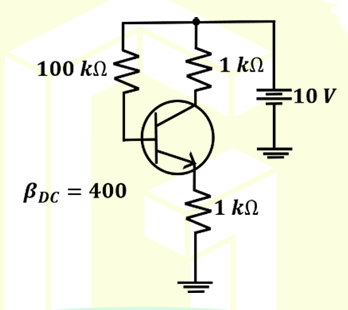
\includegraphics[width=0.3\textwidth]{figs/q60fig25.png}
\caption{Transistor circuit.}
\label{fig:q60_transistor_circuit}
\end{figure}
\hfill \textbf{(GATE PH 2025)}

\item Consider the set $\{1, x, x^2\}$. An orthonormal basis in $x \in [-1, 1]$ is formed from these three terms, where the normalization of a function $f(x)$ is defined via $\int_{-1}^1 [f(x)]^2dx = 1$. If the orthonormal basis set is $\left(\sqrt{\frac{1}{2}}, \sqrt{\frac{3}{2}}x, \frac{1}{2}\sqrt{\frac{21}{N}}(5x^2-3)\right)$, then the value of $N$ (in integer) is \underline{\hspace{3cm}}.
\hfill \textbf{(GATE PH 2025)}

\item The Hamiltonian for a one dimensional system with mass $m$, position $q$ and momentum $p$ is $H(p, q) = \frac{p^2}{2m} + q^2A(q)$, where $A(q)$ is a real function of $q$. If $m\frac{d^2q}{dt^2} = -5qA(q)$, then $\frac{dA(q)}{dq} = n\frac{A(q)}{q}$. The value of $n$ (in integer) is \underline{\hspace{3cm}}.
\hfill \textbf{(GATE PH 2025)}

\item A system of five identical, non-interacting particles with mass $m$ and spin $\frac{3}{2}$ is confined to a one-dimensional potential well of length $L$. If the lowest energy of the system is $N\frac{\pi^2\hbar^2}{2mL^2}$, the value of $N$ (in integer) is \underline{\hspace{3cm}}.
\hfill \textbf{(GATE PH 2025)}

\item A wheel of mass $4M$ and radius $R$ is made of a thin uniform distribution of mass $3M$ at the rim and a point mass $M$ at the center. The spokes of the wheel are massless. The center of mass of the wheel is connected to a horizontal massless rod of length $2R$, with one end fixed at O, as shown in the figure. The wheel rolls without slipping on horizontal ground with angular speed $\Omega$. If $\vec{L}$ is the total angular momentum of the wheel about O, then the magnitude $|\frac{d\vec{L}}{dt}| = N(MR^2\Omega^2)$. The value of $N$ (in integer) is \underline{\hspace{3cm}}.
\begin{figure}[H]
\centering
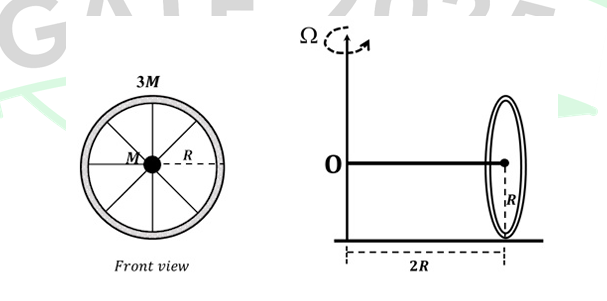
\includegraphics[width=0.6\textwidth]{figs/q64fig25.png}
\caption{Rotating and rolling wheel.}
\label{fig:q64_wheel}
\end{figure}
\hfill \textbf{(GATE PH 2025)}

\item The figure shows an opamp circuit with a 5.1 V Zener diode in the feedback loop. The opamp runs from $\pm 15$ V supplies. If a +1V signal is applied at the input, the output voltage (rounded off to one decimal place) is \underline{\hspace{3cm}}.
\begin{figure}[H]
\centering
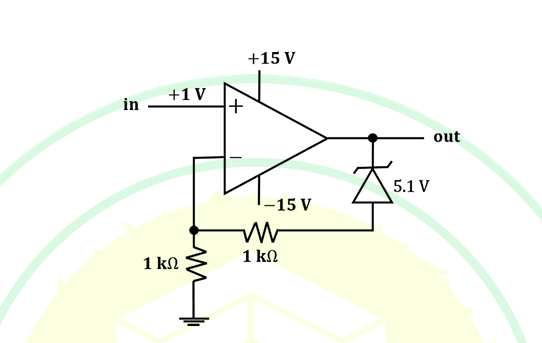
\includegraphics[width=0.5\textwidth]{figs/q65fig25.png}
\caption{Op-amp circuit with Zener diode.}
\label{fig:q65_opamp_circuit}
\end{figure}
\hfill \textbf{(GATE PH 2025)}

\end{enumerate}

\begin{center}
\textbf{END OF THE QUESTION PAPER}
\end{center}

\end{document}